This chapter introduces the elliptical PMCLP where there is no axis-parallel constraint, and the ellipses can be freely rotated. We refer to this problem as \sigla{MCER}{Maximal Covering by Ellipses with Rotation}. In comparison with MCE, this problem introduces a new variable that is responsible for determining the rotation angle of every ellipse, making MCER a more challenging problem.

\section{Definition}

An instance of the non-axis-parallel is defined exactly like the axis-parallel one on \autoref{chapter:mce}. It is given by a set of demand points $\Pp=\{p_1, \dots, p_n\}$, $p_j\in\R^2$; a list of weights $\Ww:=\{w_1, \dots, w_n\}$, with $w_j\in\R_{\ge0}$ being the weight of point $p_j$;
and $m$ ellipses given by their shape parameters $\Rr:=\{(a_1, b_1), \dots, (a_m, b_m)\}$, with $(a_j, b_j)\in\R_{>0}^2$ and $a_j>b_j$.
Additionally, to make the text more clear, we define a set of $m$ ellipses as $\E = \{E_1, \dots, E_m\}$, with $E_j\colon \R^2\times\R \mapsto \R^2$ being a function that takes the center and angle of rotation where the $j$-th ellipse is located as input, and returns its coverage region as defined by \autoref{eq:rotated_ellipse_co}.
Lastly, an instance of MCER is defined as a tuple $(\Pp, \Ww, \Rr)$.

Given an instance of $MCER$, we define $Q:=(q_1, \dots, q_m) \in \R^{2m}$ to be the centers of each ellipse, $\Theta:=(\theta_1, \dots, \theta_m) \in [0, \pi)^m$ to be the angle of rotation of each ellipse and $E_i(q_i, \theta_i)$ to be the coverage region of ellipse $E_i$ with its center at point $q_i$ rotated by angle $\theta_i$, which is given by \autoref{eq:rotated_ellipse_co}. Therefore MCER is defined as the problem of determining $Q$ and $\Theta$ (placing and rotating each ellipse) to maximize the weight of points covered by the $m$ ellipses, which is given by

\begin{equation}\label{eq:optMCEn}
\max_{Q, \Theta}{w\left(\bigcup_{i=1}^{m} \Pp \cap E_i(q_i, \theta_i)\right)}.
\end{equation}
In addition to that, we define an equivalence relation between solutions of MCER. We say that two solutions are equivalent if the set of points covered by them is the same. In other words, two solutions of MCER $(Q, \Theta)$ and $(Q', \Theta')$ are said to be equivalent if, and only if 
$$\bigcup_{j=1}^m\Pp \cap E_j(q_j', \theta_j') = \bigcup_{j=1}^m\Pp \cap E_j(q_j, \theta_j).$$

In the next section we present some results which ultimately lead up to the construction of a CLS for each facility that contains an optimal solution for MCER.

\section{Constructing a CLS}

The goal of this section is to construct a finite set of solutions, also referred to as CLS, for MCER that contains at least one optimal solution.
The main idea for doing that is to take advantage of \autoref{lema:e3p} and use the fact that there are at most six solutions for any instance of E3P.
This set of solutions is then used in the next section on the development of a $\bigO(n^{3m})$ runtime algorithm for MCER.

To begin with, a proposition is introduced which says that given an optimal solution of MCER, it is possible to find another optimal solution with two points on the border of every ellipse that is already covering at least two points.

\begin{proposicao}\label{lema:mce_2b}
	Let $(Q^*, \Theta^*)$ be an optimal solution of an instance $(\Pp, \Ww, \Rr)$ of MCER. 
	Then, for any $j\in\{1, \dots, m\}$ with $|\Pp \cap E_j(q_j^*, \theta_j^*)|\ge2$, 
	an equivalent solution $(Q', \Theta^*)$ exists, such that $|\Pp \cap \partial E_j(q_j', \theta_j^*)|\ge 2$.
\end{proposicao}

\begin{proof}
	First, the angle of rotation can be ignored as it does not change.
	
	Let $A=\Pp \cap E_j(q_j^*, \theta_j)$ be the set of points covered by the $j$-th ellipse and $X=\cap_{p \in A}E_j(p, \theta_j)$ be the region of intersection of ellipses centered at each point in $A$.

	As it was shown on \autoref{chapter:mce}, $X$ is a region that is limited by arcs of ellipses. As this region is the non-empty intersection of more than one ellipse, there are at least two of these arcs that encounter at one point, creating a vertex. Selecting any of these vertices as $q_j'$ will make $|\Pp \cap \partial E_j(q_j', \theta_j)| \ge 2$.
	
\end{proof}

What \autoref{lema:mce_2b} is saying is that any optimal solution for MCER can be transformed into an equivalent optimal solution where every ellipse that covers more than one point has two points on their border. Also, this equivalent optimal solution can be always achieved by just translating the ellipses. An example of that can be seen in \autoref{fig:ellipse-2-points}. 

Next, a notation is defined for the set of equivalent solutions of an optimal solution that has at least two points on the border of every ellipse. This helps us make the text less cluttered.

\begin{definicao}
	Let $(Q^*, \Theta^*)$ be an optimal solution for an instance $(\Pp, \Ww, \Rr)$ of MCER. We define $\Pi(Q^*, \Theta^*)$ as the set of every equivalent solution of $(Q^*, \Theta^*)$, such that for any $(Q, \Theta)\in\Pi(Q^*, \Theta^*)$, for $j\in\{1, \dots, m\}$ with $|\Pp \cap E_j(q_j^*, \theta_j^*)|\ge2$, we have $|\Pp \cap \partial E_j(q_j', \theta_j)| \ge 2$.
\end{definicao}

A lot of the ideas developed in this chapter are based on fixing two points on the border of an ellipse.
Based on that, \autoref{def:feasible_angle} introduces a new notation for angles that, given two points and an ellipse, it is possible to find a center where the ellipse rotated by that angle is placed, such that the two given points lie on its border.

\begin{figure}
	\centering
	\caption{An optimal solution before and after applying \autoref{lema:mce_2b}.}
	\includegraphics[scale=.38]{tex/figures/ellipse-2-points}
	\fautor
	\label{fig:ellipse-2-points}
\end{figure}

\begin{definicao}\label{def:feasible_angle}
	Let $E$ be the coverage region of an ellipse and $u, v \in \R^2$. An angle $\theta \in [0, \pi)$ is said to be $(E, u, v)$-feasible if there is $q \in \R^2$ such that $\{u, v\} \subset \partial E(q, \theta)$.
	In addition to that, given an instance  $(\Pp, \Ww, \Rr)$ of MCER, the set of $(E_j, u, v)$-feasible angles is referred to as 
	
	\begin{equation}
	\Phi_j(u, v) := \{\theta \in [0, \pi] : \theta \textnormal{ is a } (E_j,u,v)\textnormal{-feasible angle}\}.
	\end{equation}
\end{definicao}

In \autoref{fig:feasible-angle} two examples for \autoref{def:feasible_angle} are shown. The example with a solid contour shows two ellipses rotated by $\pi/4$ with the two given points on its border, making $\pi/4$ a $(E, u, v)$-feasible angle.
The other example, with a dashed contour, presents a case where an ellipse rotated by $\pi/2$ is not able to have the two points on its border, no matter where it is placed; because of that, $\pi/2$ is said to be a not $(E, u, v)$-feasible angle.

\begin{figure}[H]
	\centering
	\caption{A $(E, u, v)$-feasible angle and a not $(E, u, v)$-feasible angle.}
	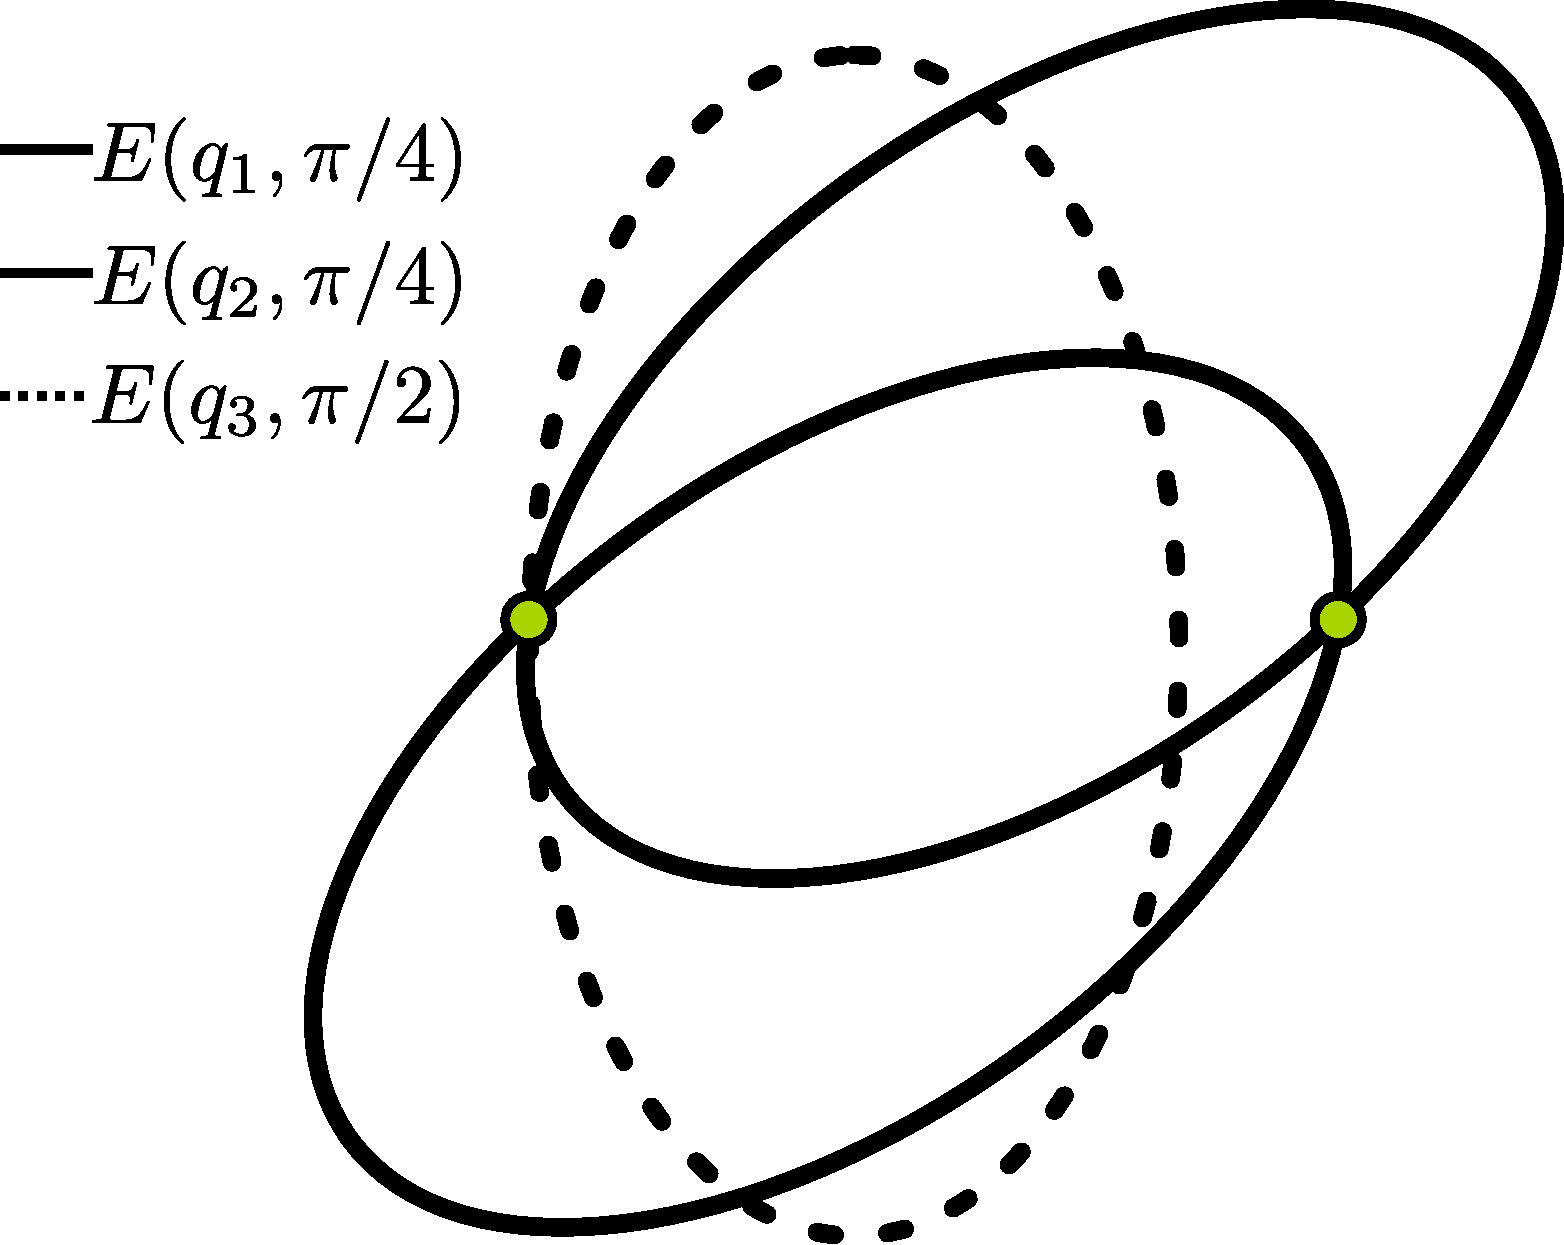
\includegraphics[scale=.33]{tex/figures/feasible-angle2}
	\fautor
	\label{fig:feasible-angle}
\end{figure}

Following that, we present a lemma that, given an optimal solution, it says that for any ellipse that covers more than two points, an equivalent solution exists with at least one of the two properties:
\begin{itemize}
	\item Three points lie on the ellipse's border.
	\item Two points lie on the ellipse's border, for any feasible angle.
\end{itemize}

\begin{lema}\label{lema:3pnts}
Let $(Q^*, \Theta^*)$ be an optimal solution of an instance $(\Pp, \Ww, \Rr)$ of MCER; $j\in\{1, \dots, m\}$, such that $|\Pp \cap E_j(q_j^*, \theta_j^*)|>2$; $(Q', \Theta')\in\Pi(Q^*, \Theta^*)$; and $\{u, v\}\subset \partial E_j(q_j', \theta_j')$.

If, for every equivalent solution $(\hat{Q}, \hat{\theta})$, $|\Pp\cap \partial E_j(\hat{q}_j, \hat{\theta}'_j)| < 3$, then for all $\theta\in\Phi_j(u,v)$, there exists $q\in\R^2$, such that $\{u, v\} \subset \partial E_j(q, \theta)$ and $\Pp \cap E_j(q^*_j, \theta^*_j) = \Pp \cap E_j(q, \theta)$.

\end{lema}

\begin{proof}
	According to \autoref{lema:mce_2b}, there exists $\{u, v\} \subset \Pp \cap E_j(q^*_j, \theta^*_j)$, such that an equivalent optimal solution $(Q', \Theta')$ exists with $u$ and $v$ on the border of $E_j(q_j', \theta_j^*)$. Therefore, $\theta_j^*\in\Phi_j(u,v)$.
	
	Now suppose that $u$ and $v$ have the same $y$-coordinate, that is, the angle between them is $0$. If they do not, a rotation can be applied to make them have the same $y$-coordinate. Then, the first thing we are proving is that $\Phi_j(u, v) = [0, 2\alpha]$ for a specific case that any instance can be transformed into using translation and rotation on every element of $\Pp$.
	
	In \autoref{chapter:definitions}, a function $L\colon \R \to \R_{\ge0}$ was defined in \autoref{eq:function-l}. This function takes the angular coefficient $m\in\R$ and, considering the family of lines parallel to the one described by $y=mx$, returns the maximum squared distance between two intersection points of a line in that family and an axis-parallel ellipse centered at the origin.
	
	To use those results here, we need to consider the ellipse to be fixed at the origin and axis-parallel, and instead, rotate the points in $\Pp$. 
	
	Let $\theta \in [0, \pi]\setminus\{\pi/2\}$, and $u', v'$ be the points $u, v$ after a rotation by $\theta$. Then, if $L(\tan{\theta}) \ge ||v-u||_2^2$, it is possible to apply a translation to $u',v'$, such that they end up in the border of the fixed ellipse. This means that, it is possible to find an angle of rotation and a center to place $E_j$, such that it has $u, v$ on its border. 
	
	Now we use some properties of function $L$ whose details are given in \autoref{chapter:definitions}.
	Defining $l(\theta)=L(\tan{\theta})$, with $l:[0, \pi]\setminus\{\pi/2\}$, we can say that
	
	\begin{itemize}
		\item $l$ is decreasing in $[0, \pi/2)$ because $L$ is decreasing in $[0, \infty)$. Therefore, if there is $\alpha\in[0, \pi/2)$, such that $l(\alpha) = ||v-u||_2^2$, then $l(\theta)>||v-u||_2^2$, for $\theta\in(\alpha, \pi/2)$. That implies $[0, \alpha] \subset \Phi_j(u,v)$.
		\item $l(\theta) = l(\pi-\theta)$ because $L$ is an even function. Therefore, if there is $\alpha\in[0, \pi/2)$, such that $l(\alpha) = ||v-u||_2^2$, then $l(\theta)>||v-u||_2^2$, for $\theta\in(\pi/2,\pi-\alpha)$. That implies $[\pi-\alpha, \pi] \subset \Phi_j(u,v)$.
	\end{itemize}
	We then conclude that $\Phi_j(u, v) = [0, \alpha]\cup [\pi-\alpha, \pi]$, and, of course, in the case that there is no $\alpha\in[0, \pi/2)$, such that $l(\alpha)=||v-u||_2^2$, we have $\Phi_j(u,v)=[0, \pi]$.
	From that, if we rotate every point in $\Pp$ by $\pi-\alpha$, we obtain $\Phi_j(u,v)=[0, 2\alpha]$.
	
	With this result in hands, we can use a continuity argument to complete our proof as follows.
	Let $\delta : \Phi_j(u,v) \mapsto \R^2$ be a continuous function which takes an angle $\theta\in\Phi_j(u,v)$ and returns a center, such that $\{u,v\} \subset \partial E_j(\delta(\theta), \theta)$, and, from solution $(Q', \Theta')$, $\delta(\theta_j') = q_j'$.
	In general, for any angle in $\Phi_j(u,v)$, there are two possible centers that make $\{u,v\} \subset \partial E_j(\delta(\theta), \theta)$ (see \autoref{fig:feasible-angle} for an example), however, as $\delta(\theta_j') = q_j'$, $\delta$ is well-defined. This is shown in \autoref{fig:lema-3-points} where $\delta$ is plotted for the whole interval $\Phi_j(u,v)$.
	
	Let $w\in \Pp \cap E_j(q_j^*, \theta_j^*) \setminus \{u,v\}$, then we define $f_w  : \R^3 \mapsto \R_{\ge0}$ to be a function that takes a center point $q$ and an angle of rotation $\theta$, and returns the elliptical distance between $w$ and $E_j(q, \theta)$ as defined by the left-and-side of \autoref{eq:rotated_ellipse}.
	
	For all $w\in \Pp \cap E_j(q_j^*, \theta_j^*)\setminus \{u,v\}$, we have that $f_w(q_j', \theta_j^*) < 1$. We then define a function $g_w\colon \Phi_j(u,v) \mapsto \R_{\ge0}$ as $g_w(\theta) = f_w(\delta(\theta), \theta)$. As $g_w$ is a composition of continuous functions, it is also continuous.
	
	Therefore, for any $\theta\in\Phi_j(u,v)$, if a point $w \in \Pp \cap E_j(q_j^*, \theta_j^*)\setminus\{u,v\}$ is not covered by $E_j(\delta(\theta), \theta)$, it must have $g_w(\theta)>1$. Then, by continuity, another angle $\hat{\theta} \in(\theta_j^*, \theta)$ must exist, such that $g_w(\hat{\theta})=1$, which means that $w\in \partial E_j(\delta(\hat{\theta}), \hat{\theta})$, contradicting the hypothesis. The same can be said about a point that enters the coverage of $E_j(\delta(\theta), \theta)$.
\end{proof}

%\begin{figure}[H]%
%	\centering%
%	\caption{Every ellipse that contains two points for a fixed angle of %rotation.}
%	\includegraphics[scale=.36]{tex/figures/2point-ellipse}
%	\fautor
%	\label{fig:2point-ellipse}
%\end{figure}

What \autoref{lema:3pnts} is saying is that, for every ellipse in an instance of MCER, unless an equivalent optimal solution with three points on its border exits, the angle of rotation can practically be ignored. Because of that, it will be shown that we can construct a CLS which is finite and also contains an optimal solution.

In \autoref{fig:lema-3-points} a visualization of \autoref{lema:3pnts} is presented.
An initial optimal solution is given by the dashed-border ellipse, and its center, represented by a star point. From it, the continuous function $\delta$ is defined by moving the ellipse through the rotation angles in $\Phi_j(u,v)$ while maintaining $u, v$ on its border. Ten angles were chosen from $\Phi_j(u,v)$ to be shown in \autoref{fig:lema-3-points}, among those were $0$ and $\max\{\Phi_j(u,v)\}$; their corresponding ellipses are displayed with solid-line borders.
Consistently with \autoref{lema:3pnts}, the points in $\Pp \setminus \{u, v, w\}$ stay within the ellipse's cover for any angle of rotation, and, for point $w$, there exists an angle, such that it is on the ellipse's border.  

\begin{figure}[H]
	\centering
	\caption{A visualization of \autoref{lema:3pnts}.}
	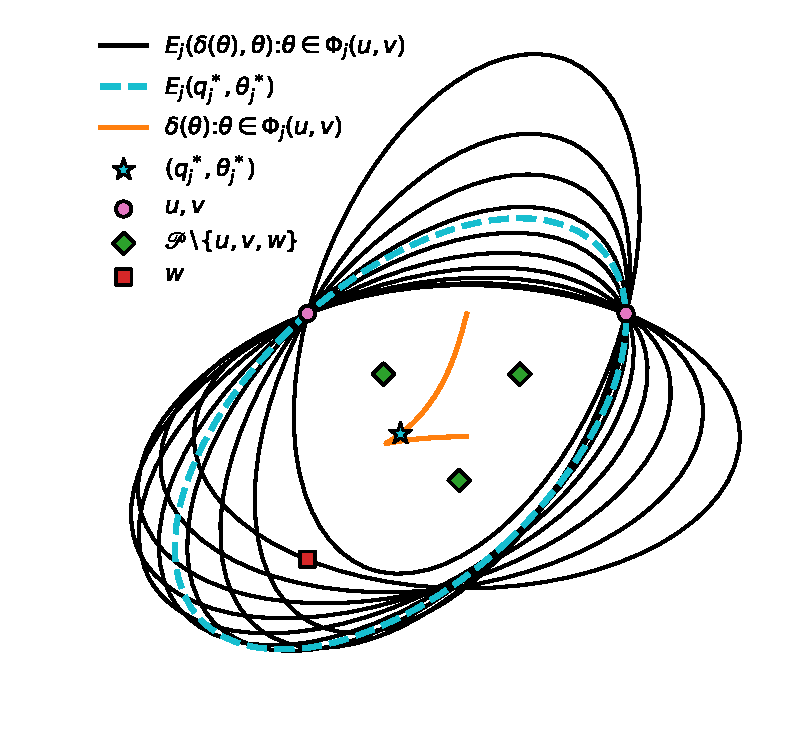
\includegraphics[scale=.6]{tex/figures/lema-3-points}
	\fautor
	\label{fig:lema-3-points}
\end{figure}

Let $(Q^*, \Theta^*)$ be an optimal solution of an instance $(\Pp, \Ww, \Rr)$ of MCER. We will define a set $\Omega(\Pp, \Ww, \Rr)$ and show that there exists an equivalent solution $(Q', \Theta')$ to  $(Q^*, \Theta^*)$, such that $(Q', \Theta') \in \Omega(\Pp, \Ww, \Rr)$. This is the same thing as showing that $\Omega(\Pp, \Ww, \Rr)$ contains an optimal solution for the instance $(\Pp, \Ww, \Rr)$.
The whole set $\Omega(\Pp, \Ww, \Rr)$ is constructed from a set of solutions for every ellipse. Let $j\in\{1, \dots, m\}$, we denote by $S_j$ the CLS for the $j$-th ellipse; its construction is broken into three separated cases denoted by $S_j^{(1)}$, $S_j^{(2)}$, and $S_j^{(3)}$. Next, we define them precisely.

\subsection{First case}

This is the case where $|E_j(q_j^*, \theta_j^*)|=1$, that is, the $j$-th ellipse only covers one point. 
This case is not treated by any of the previous results presented in this chapter. Nevertheless, taking this possibility into account can be done by including solutions in $S_j$ that are guaranteed to cover at least one point. This is represented by
\begin{equation}
	S_j^{(1)} = \bigcup_{u \in \Pp} \{(u, 0)\}.
\end{equation}

\subsection{Second case}

The second and third cases are addressed by \autoref{lema:3pnts}. 
Consider the second case to be the one where the $j$-ellipse covers more than one point and there is no equivalent solution with three points on the its border. 
By \autoref{lema:3pnts}, $(Q^*, \Theta^*)$ can be represented by a solution that has some pair of points $u, v$ on the ellipse's border, and is rotated by some angle in $\Phi_j(u,v)$. 
As only one angle is needed, we define $\theta_{uv}$ as the angle that makes the major-axis of the ellipse to be aligned with the line that passes through $u$ and $v$; this angle surely is in $\Phi_j(u,v)$ as the longest segment that crosses an ellipse is its major-axis.
Having said that, we refer to $S_j^{(2)}$ the set of possible solutions that takes this case into account; we define it as
\begin{equation}
S_j^{(2)} = \bigcup_{\{u, v\} \subset \Pp} \{(q, \theta_{uv})\in \R^2\times\R: \{u,v\} \subset \partial E_j(q, \theta_{uv})\}.\\
\end{equation}
For a pair of points $u, v$, determining every ellipse with a fixed rotation angle that has $u$ and $v$ on its border is equivalent to determining the intersection points of two axis-parallel ellipses with the same shape parameters. This problem is discussed with great detail in \autoref{section:ellipses_intersection}.

\subsection{Third case}

The only case left is the one where there is an equivalent solution with three points on the $j$-th ellipse's border. We call this set of possible solutions $S_j^{(3)}$, and define it as
\begin{equation}
	S_j^{(3)} = \bigcup_{\{u, v, w\} \subset \Pp} \{(q, \theta)\in \R^2\times\R: \{u, v, w\} \subset \partial E_j(q, \theta)\}.
\end{equation}
Determining the set $S_j^{(3)}$ can be done using the results from \autoref{chapter:e3p} for every triplet of points.

Finally, we define the CLS for the $j$-th ellipse as $S_j = S_j^{(1)} \cup S_j^{(2)} \cup S_j^{(3)}$, and the set of possible solutions of an instance of MCER as
\begin{equation}\label{eq:omega}
\Omega(\Pp, \Ww, \Rr) = \{(Q, \Theta)\in \R^{2m}\times\R^m \colon (q_j, \theta_j) \in S_j \textnormal{ for all } j\in\{1, \dots, m\}\}.
\end{equation}

\begin{theorem}\label{th:mcer}
	Let $(\Pp, \Ww, \Rr)$ be an instance of MCER, and $\Omega(\Pp, \Ww, \Rr)$ be a set of solutions defined by \autoref{eq:omega}. Then there exists an optimal solution $(Q^*, \Theta^*) \in \Omega(\Pp, \Ww, \Rr)$, and $|\Omega(\Pp, \Ww, \Rr)|=\bigO(n^{3m})$.	
\end{theorem}

\begin{proof}
	For every $j \in \{1, \dots, m\}$, by \autoref{lema:3pnts}, any optimal solution that covers more than one point can be transformed into one that is in $S_j^{(2)}$ or in $S_j^{(3)}$.
	If an optimal solution covers only one point, it can be transformed into another one that is in $S_j^{(1)}$.
	
	From \autoref{section:ellipses_intersection}, we can conclude that $|S_j^{(2)}|\le 2\binom{n}{2} = \bigO(n^2)$.
	By \autoref{lema:e3p}, we have that $|S_j^{(3)}| \le 6\binom{n}{3} = \bigO(n^3)$.
	Therefore, $|S_j|=\bigO(n^3)$, and as $|\Omega(\Pp, \Ww, \Rr)|= |S_1|\times|S_2|\times\dots\times|S_m|$, we have $|\Omega(\Pp, \Ww, \Rr)|=\bigO(n^{3m})$.
\end{proof}

\section{An algorithm for MCER}

In this section we describe an algorithm for MCER that does a complete search on the CLS of each ellipse.

Firstly, we describe an algorithm that constructs a CLS for a given ellipse.
Let $E$ be the coverage region of an ellipse with shape parameters $(a, b)$. We assume that in \autoref{algoritmo:mcer1}, the procedure $e2p(u, v, a, b)$ returns every $(q, \theta) \in \R^2\times\R$, such that, $\{u, v\}\subset \partial E(q, \theta)$, and $\theta$ is an rotation angle that makes $E$'s major-axis parallel to the line defined by $u$ and $v$. Also, the procedure $e3p$ called in \autoref{algoritmo:mcer1} is defined in \autoref{algoritmo:e3p}.

\begin{algoritmo}
	\caption{An algorithm that constructs a CLS for a given ellipse.}\label{algoritmo:mcer1}
	\begin{algorithmic}[1]
		\Require{A set of points $\Pp=\{p_1,\dots,p_n\}$, and an ellipse's shape parameters $(a, b)$.}
		
		\Ensure{A CLS for the ellipse with shape parameters $(a, b)$ considering the demand set $\Pp$.}
		
		\item[]
		
		\Procedure{CLS-MCER}{$\Pp, a, b$}
		\State $S \gets \{\}$
		
		\For {$u \in \Pp$}
		\State $S \gets S \cup \{(u, 0)\}$
		\EndFor
		
		\For {$\{u, v\} \in \Pp$}
		\State $S \gets S \cup e2p(u, v, a, b)$
		\EndFor
		
		\For{$\{u, v, w\} \in \Pp$}
		\State $S \gets S \cup e3p(u, v, a, b)$ \Comment{Defined in \autoref{algoritmo:e3p}.}
		\EndFor
		
		\State \Return $S$
		\EndProcedure
	\end{algorithmic}
\end{algoritmo}

After that, we define \autoref{algoritmo:mcer} which takes an instance $(\Pp, \Ww, \Rr)$ of MCER, and returns an optimal solution for it.
Even though it is based on \autoref{th:mcer}, the set of solutions $\Omega(\Pp, \Ww, \Rr)$ is not explicitly built in \autoref{algoritmo:mcer}. Instead, a complete search is done by backtracking the CLS of every ellipse returned by procedure CLS-MCER.

Two procedures are defined in \autoref{algoritmo:mcer}. The first one, called $MCER$, returns an optimal solution for an instance $(\Pp, \Ww, \Rr)$ using the second procedure $MCER_{bt}$. This second procedure is responsible for the backtracking and takes two additional parameters $j\in\{1, \dots, m\}$, which represents the index of the ellipse that $MCER_{bt}$ is currently processing, and $Z\subset \Pp$, which represents the set of points that have not been covered by the ellipses already processed by $MCER_{bt}$.


\begin{algoritmo}
	\caption{Algorithm for MCER}\label{algoritmo:mcer}
	\begin{algorithmic}[1]
		\Require{A set of points $\Pp=\{p_1,\dots,p_n\}$, a list of weights $\Ww=\{w_1, \dots, w_n\}$, and a list of shape parameters $\Rr=\{(a_1, b_1), \dots, (a_m, b_m)\}$.}
		
		\Ensure{An optimal solution for the given instance of MCER.}
		
		\item[]
		\Procedure{$MCER$}{$\Pp, \Ww, \Rr$}
		\State \Return $MCER_{bt}(\Pp, \Ww, \Rr, 1)$
		\EndProcedure
		
		\item[]
		
		\Procedure{$MCER_{bt}$}{$Z, \Ww, \Rr, j$}
		\If{$j = m+1$}
		\State \Return $0$
		\EndIf
		
		\State $ans \gets 0$
		\State $(q_{j}^*, \dots, q_m^*); (\theta_{j}^*, \dots, \theta_m^*) \gets (0, \dots 0); (0, \dots, 0)$ \Comment{Setting to $0$ as a default value.}
		
		\State $S_j \gets \textnormal{CLS-MCER}(Z, a_j, b_j)$

		
		\For{$(q_j, \theta_j) \in S_j$}
		\State $Cov \gets \Pp \cap E_j(q_j, \theta_j)$
		
		\State $(q_{j+1}, \dots, q_m); (\theta_{j+1}, \dots, \theta_m) \gets  MCER_{bt}(Z\setminus Cov, \Ww, \Rr, j+1)$
		
		
		\State $Cov \gets \bigcup_{k=j}^m \Pp \cap E_k(q_k, \theta_k)$
		\If {$w(Cov) > ans$}
			\State $ans \gets w(Cov)$
			%\State $((q_{j}^*,\theta_{j}^*); \dots; (q_m^*, \theta_m^*)) \gets ((q_{j},\theta_{j}); \dots; (q_m, \theta_m))$
			
			\State $(q_{j}^*, \dots, q_m^*); (\theta_{j}^*, \dots, \theta_m^*) \gets (q_{j}, \dots, q_m); (\theta_{j}, \dots, \theta_m)$
		\EndIf
		\EndFor
		
		\State \Return $(q_{j}^*, \dots, q_m^*); (\theta_{j}^*, \dots, \theta_m^*)$
		\EndProcedure
	\end{algorithmic}
\end{algoritmo}

\begin{corolario}
	\autoref{algoritmo:mcer} takes $\bigO(n^{3m})$ computations and returns an optimal solution for an instance of MCER.
\end{corolario}

\begin{proof}
	For every $j\in\{1, \dots, m\}$, unless $Z=\{\}$, when choosing the center and angle of rotation for the $j$-th ellipse, \autoref{algoritmo:mcer} does not consider any $(q_j, \theta_j) \in \R^2 \times \R$, such that $Z \cap E_j(q_j, \theta_j) = \{\}$. Apart from those solutions, which are non-optimal, \autoref{algoritmo:mcer} considers every solution in $\Omega(\Pp, \Ww, \Rr)$.
\end{proof}

In \autoref{fig:AB120} a solution return by \autoref{algoritmo:mcer} for the instance AB120 taken from \citeonline{andreta} is displayed. The exact method developed by \citeonline{andreta}, for this instance, could not obtain an optimal solution within the established time limit, however, comparing with the solution obtained by our algorithm, their heuristic method does find an optimal solution. In the next chapter, we give more details about the solutions found by our algorithm, along with the proposal of some new instances for MCER and MCER-$k$.


\begin{figure}[H]
	\centering
	\caption{An optimal solution for the instance AB120.}
	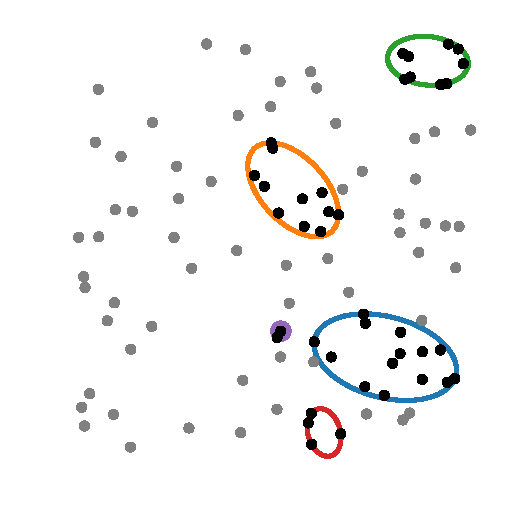
\includegraphics[scale=.5]{tex/figures/AB120}
	\fautor
	\label{fig:AB120}
\end{figure}

\subsection{Adding facility cost}

In this section, we consider the extended version of MCER where each facility has a cost assigned to it and exactly $k$ of them must be used in a solution. We refer to this version of the problem as \sigla{MCER-$k$}{Maximum Covering by Ellipses with Rotation and a $k$-constraint}. 

An instance of MCER-$k$ has the same parameters as MCER plus a list of costs \mbox{$\Cc:=\{c_1, \dots, c_m\}$}, with $c_j\in\R_{>0}$ being the cost of the $j$-th facility; and $k\in\mathbb{N}$, $k\le m$.

A solution for MCER-$k$ is given by $(I, Q, \Theta)$, with $I:=\{i_1, \dots, i_k\}\subset \{1, \dots, m\}$; \\\mbox{$Q:=(q_1, \dots, q_k)\in\R^{2k}$}, with $q_j$ being the center of the $i_j$-th ellipse; and \mbox{$\Theta:=(\theta_1, \dots, \theta_k) \in [0, \pi)^k$}, with $\theta_j$ being the angle of rotation of the $i_j$-th ellipse. An optimal solution of MCER-$k$ is given by the optimization problem

\begin{equation*}
	\max_{I, Q, \Theta} w\left(\bigcup_{j=1}^k \Pp \cap E_{i_j}(q_j, \theta_j)\right).
\end{equation*}

Then, in the same way that it is done in \autoref{chapter:mce}, we introduce \autoref{algoritmo:mcer-k} for MCER-$k$ that uses \autoref{algoritmo:mcer} for every $I:=\{i_1, \dots, i_k\} \subset \{1, \dots, m\}$. Therefore, \autoref{algoritmo:mcer-k} returns an optimal solution for MCER-$k$ in $\bigO(\binom{m}{k}n^{3k}) = \bigO(n^{4m})$ time.

\begin{algoritmo}
	\caption{Algorithm for MCER-$k$}\label{algoritmo:mcer-k}
	
	
	\begin{algorithmic}[1]
		\Require{A set of points $\Pp=\{p_1,\dots,p_n\}$, a list of weights $\Ww=\{w_1, \dots, w_n\}$, a list of shape parameters $\Rr=\{(a_1, b_1), \dots, (a_m, b_m)\}$, a list of costs $\Cc=\{c_1, \dots, c_m\}$, and $k\in \mathbb{N}$.}
		\Ensure{An optimal solution for MCER-$k$.}
		
		\item[]
		
		\Procedure{MCER-$k$}{$\Pp, \Ww, \Rr, \Cc, k$}
		\State $I^* = \{i_1^*, \dots, i_k^*\}\gets \{1, \dots, k\}$
		\State $Q^* = (q_1^*, \dots, q_k^*) \gets (0, \dots, 0)$
		\State $\Theta^* = (\theta_1^*, \dots, \theta_k^*) \gets (0, \dots, 0)$
		
		\ForAll{$I=\{i_1, \dots, i_k\} \subset \{1, \dots, m\}$}
		
		\State $\Rr' \gets \{(a_j, b_j) \in \Rr: j \in I\}$
		\State $(q_1, \dots, q_k); (\theta_1, \dots, \theta_k) \gets MCER(\Pp, \Ww, \Rr')$
		
		\If{$w(\bigcup_{j=1}^k \Pp \cap E_{i_j}(q_j, \theta_j)) - \sum_{j\in I} c_j > w(\bigcup_{j=1}^k \Pp \cap E_{i_j^*}(q_j^*, \theta_j^*)) - \sum_{j\in I^*}c_{j}$}
		\State $Q^* \gets (q_1, \dots, q_k)$
		\State $\Theta^* \gets (\theta_1, \dots, \theta_k)$
		\State $I^* \gets I$
		\EndIf
		\EndFor
		
		\State \Return $I^*, Q^*, \Theta^*$
		\EndProcedure
	\end{algorithmic}
\end{algoritmo}


\subsection{Improvements and implementation details}

Some improvements can be made in the implementation of \autoref{algoritmo:mcer}.
Instead of calling procedure CLS-MCER every time in the backtracking routine, it is suggested that it is done outside in a pre-processing phase.

Let $(Q, \Theta)$ and $(Q', \Theta')$ be two solutions of MCER. If, for any $j \in \{1, \dots, m\}$, we have $\Pp \cap E_j(q_j', \theta_j') \subset \Pp \cap E(q_j, \theta_j)$, solution $(Q', \Theta')$ can be dismissed. This can be done in the CLS-MCER procedure in \autoref{algoritmo:mcer1}. 

In our implementation we use the same approach used in \citeonline{andreta}. When constructing the CLS for the $j$-th ellipse, a tree-like data structure is utilized to verify if a solution $(q, \theta)$ covers a subset of another solution or not.

Keeping an upper-bound for the solution during the backtracking in \autoref{algoritmo:mcer} can also provide a good improvement in practice. Let $z_j = \max_{(q, \theta) \in S_j} w(\Pp \cap E_j(q, \theta))$, and $OPT$ the value of an optimal solution. When the algorithm chooses $(q_j, \theta_j) \in S_j$ as the solution for the $j$-th ellipse, we have

\begin{equation}
OPT \le w\left(\bigcup_{k=1}^{j} \Pp \cap E_k(q_k, \theta_k)\right) + \sum_{k=j+1}^m z_k.
\end{equation}
This upper-bound is easy to compute as $\{z_1, \dots, z_m\}$ can be pre-processed, and the weight of every point covered so far in the backtrack can be obtained by adding another parameter to the $MCER$ procedure.

In the next chapter, we present the results of numerical experiments for MCER and MCER-$k$ and compare them with the results published in \citeonline{andreta}.